\documentclass[12pt]{article}

\usepackage{parskip,amsthm,amsmath,amsfonts,amssymb}
\usepackage{multicol,cancel}
\usepackage[shortlabels]{enumitem}
\usepackage[letterpaper,margin=1in,bottom=0.7in]{geometry}
\newcommand{\dd}[2]{\dfrac{d #1}{d #2}}
\newcommand{\ddd}[2]{\dfrac{d^2 #1}{d #2^2}}
\newcommand{\pd}[2]{\dfrac{\partial #1}{\partial #2}}
\newcommand{\ppd}[2]{\dfrac{\partial^2 #1}{\partial #2^2}}
\newcommand{\ppdd}[3]{\dfrac{\partial^2 #1}{\partial #2\partial #3}}
\newcommand{\brf}[2]{\left(\frac{#1}{#2}\right)}
                       % Bracket-frac, e.g. for (n\pi x/L) in Fourier series
\newcommand{\fsin}[1]{\sin\brf{#1 \pi x}{L}}
\newcommand{\fcos}[1]{\cos\brf{#1 \pi x}{L}}
\newcommand{\fsint}[1]{\sin\brf{#1 \pi t}{L}}
\newcommand{\fcost}[1]{\cos\brf{#1 \pi t}{L}}
\newcommand{\RR}{\mathbf{R}}
\newcommand{\CC}{\mathbf{C}}
\newcommand{\ZZ}{\mathbf{Z}}
\newcommand{\mks}[1]{\begin{flushright}(#1 marks)\end{flushright}}

\usepackage{tikz}
\newcommand{\lapl}[6]{
\begin{tikzpicture}[scale=2]
  \draw (0,0) -- (0,1);
  \draw (0,1) -- (1,1);
  \draw (1,1) -- (1,0);
  \draw (1,0) -- (0,0);
  \node at (0.5,0.5) {$#6$};
  \node [below] at (0.5,0) {$#1(x,0)=#2$};
  \node [above] at (0.5,1) {$#1(x,\pi)=#3$};
  \node [left] at (0,0.5) {$#1(0,y)=#4$};
  \node [right] at (1,0.5) {$#1(\pi,y)=#5$};
\end{tikzpicture}
}

\newcommand{\onelapl}[6]{
\begin{tikzpicture}[scale=2]
  \draw (0,0) -- (0,1);
  \draw (0,1) -- (1,1);
  \draw (1,1) -- (1,0);
  \draw (1,0) -- (0,0);
  \node at (0.5,0.5) {#6};
  \node [below] at (0.5,0) {$#1(x,0)=#2$};
  \node [above] at (0.5,1) {$#1(x,1)=#3$};
  \node [left] at (0,0.5) {$#1(0,y)=#4$};
  \node [right] at (1,0.5) {$#1(1,y)=#5$};
\end{tikzpicture}
}


\newcommand{\mlapl}[6]{
\begin{tikzpicture}[scale=2]
  \draw (0,0) -- (0,1);
  \draw (0,1) -- (1,1);
  \draw (1,1) -- (1,0);
  \draw (1,0) -- (0,0);
  \node at (0.5,0.5) {#1};
  \node [below] at (0.5,0) {$#6(x,0)=#2$};
  \node [above] at (0.5,1) {$#6(x,\pi)=#3$};
  \node [left] at (0,0.5) {$#6(0,y)=#4$};
  \node [right] at (1,0.5) {$#6(\pi,y)=#5$};
\end{tikzpicture}
}
\newcommand{\laplneu}[6]{
\begin{tikzpicture}[scale=2]
  \draw (0,0) -- (0,1);
  \draw (0,1) -- (1,1);
  \draw (1,1) -- (1,0);
  \draw (1,0) -- (0,0);
  \node at (0.5,0.5) {#6};
  \node [below] at (0.5,0) {$#1(x,0)=#2$};
  \node [above] at (0.5,1) {$#1(x,\pi)=#3$};
  \node [left] at (0,0.5) {$\partial_x#1(0,y)=#4$};
  \node [right] at (1,0.5) {$\partial_x#1(\pi,y)=#5$};
\end{tikzpicture}
}

\theoremstyle{remark}
\newtheorem{rmk}{Remark}

\theoremstyle{definition}
\newtheorem{question}{Question}
\newtheorem{answer}{Answer}


%%%%%%%%%%%%%%%%%% Add extra space before theorems

\begingroup 
\makeatletter 
\@for\theoremstyle:=definition,remark,plain,TheoremNum\do{% 
\expandafter\g@addto@macro\csname th@\theoremstyle\endcsname{% 
\addtolength\thm@preskip\parskip 
}% 
} 
\endgroup 


\title{Methods 3 - Question Sheet 4}
\author{J. Evans}
\date{}


\begin{document}
\maketitle

\begin{question}(13 marks for * parts)\\
Solve the Euler-Lagrange equation for the following variational problems; you may use Beltrami's identity, where appropriate.
\begin{enumerate}[(a)]
\item * $\int_0^1\left(x^2y+\frac{(y')^2}{2}\right)dx$ subject to $y(0)=y(1)=0$.
\item * $\int_0^1\sqrt{y(1+(y')^2)}dx$ (the general solution - leave constants undetermined).
\item $\int_0^1\sqrt{(1+y)(1+(y')^2)}dx$ (the general solution - leave constants undetermined).
\item $\int_0^{\pi/4}(y')^2\cos^2 x dx$ subject to $y(0)=0$, $y(\pi/4)=1$.
\item $\int_0^{\pi}\left((y')^2+(\cos^2x-\sin x)y^2\right)dx$ subject to $y(0)=y(\pi)=1$ {\em (Hint: Compute $\ddd{(e^{\sin x})}{x}$.)}
\end{enumerate}
\end{question}

\iffalse
\begin{answer}
\begin{enumerate}[(a)]
\item * We must use the full Euler-Lagrange equation
\[\dd{}{x}\pd{L}{y'}=\pd{L}{y}\]
\mks{1}
as the integrand depends on all the variables $x,y,y'$. We have $\pd{L}{y'}=y'$ and $\pd{L}{y}=x^2$ therefore the Euler-Lagrange equation is
\[y''=x^2\]
\mks{2}
which integrates up twice to give $y'=x^3/3+C$ and $y=x^4/12+Cx+D$.
\mks{2}
The boundary conditions give $D=0$ and $C+1/12=0$ so $y=(x^4-x)/12$.
\mks{1}
\item * Since the integrand $L=\sqrt{y(1+(y')^2)}$ has no explicit $x$-dependence we can use Beltrami's identity,
\[L-y'\pd{L}{y'}=C\]
\mks{1}
where $C$ is constant. This gives
\begin{align*}
C&=\sqrt{y(1+(y')^2)}-y'\frac{\sqrt{y}y'}{\sqrt{1+(y')^2}}\\
 &=\sqrt{\frac{y}{1+(y')^2}}\left(1+(y')^2-(y')^2\right)\\
 &=\sqrt{\frac{y}{1+(y')^2}}
\end{align*}
\mks{2}
so
\[y'=\sqrt{\frac{y}{C^2}-1}.\]
Dividing by the RHS and integrating gives
\[\int\frac{Cdy}{\sqrt{y-C^2}}=x+D.\]
\mks{2}
You can do the integral by substituting $y=C^2\sec^2u$ or by spotting that $d\sqrt{y-C^2}=\frac{dy}{2\sqrt{y-C^2}}$ the result is
\[2C\sqrt{y-C^2}=x+D\]
\mks{2}
or
\[y=\left(\frac{x+D}{2C}\right)^2+C^2.\]
\item As usual we can use Beltrami and we get
\[\sqrt{(1+y)(1+(y')^2)}-\sqrt{(1+y)}\frac{(y')^2}{\sqrt{1+(y')^2}}=C\]
or
\[\sqrt{\frac{1+y}{1+(y')^2}}=C\]
which rearranges to give
\[Cy'=\sqrt{y+1-C^2}.\]
Dividing by the RHS and integrating gives
\[\int\frac{Cdy}{\sqrt{y+1-C^2}}=x+D.\]
As in (b), we see that $d\sqrt{y+1-C^2}=dy/2\sqrt{y+1-C^2}$ so the integral is
\[2C\sqrt{y+1-C^2}=x+D.\]
This rearranges to give $y=C^2-1+\left(\frac{x+D}{2C}\right)^2$.
\item The Euler-Lagrange equation for this functional is
\[0=\dd{}{x}\pd{L}{y'}=\dd{}{x}(2y'\cos^2x)=0\]
so we get $y'\cos^2 x=C$ for some constant $C$. Therefore $y'=C\sec^2x$ and $y=C\tan x+D$. The boundary conditions give $D=0$ and $C=1$ so the solution is $y=\tan x$.
\item We have
\[\dd{}{x}\pd{L}{y'}=2y'',\quad\pd{L}{y}=2(\cos^2x-\sin x)y\]
so the Euler-Lagrange equation for this functional is
\[y''=2(\cos^2x-\sin x)y.\]
The hint tells us to compute
\[\ddd{(e^{\sin x})}{x}=\dd{}{x}\left((\cos x)e^{\sin x}\right)=\cos^2xe^{\sin x}-\sin xe^{\sin x}\]
so certainly $y=e^{\sin x}$ satisfies the Euler-Lagrange equation. It also satisfies the boundary conditions $y(0)=y(\pi)=e^0=1$.
\end{enumerate}
\end{answer}

\newpage
\fi

\bigskip

\begin{question}(7 marks)\\
\begin{multicols}{2}
Consider the functional
\[F(y)=\int_a^b\frac{\sqrt{1+(y')^2}}{y}dx\]
for functions $y$ satisfying $y(a)=A$, $y(b)=B$. Find the general solution to the Euler-Lagrange equation for this functional and show that if $y$ is a solution then the graph
\[\left\{(x,y(x))\ :\ x\in[a,b]\right\}\]
is a segment of a circle
\[y^2+(x-C)^2=D\]
centred on the $x$-axis.

\begin{center}
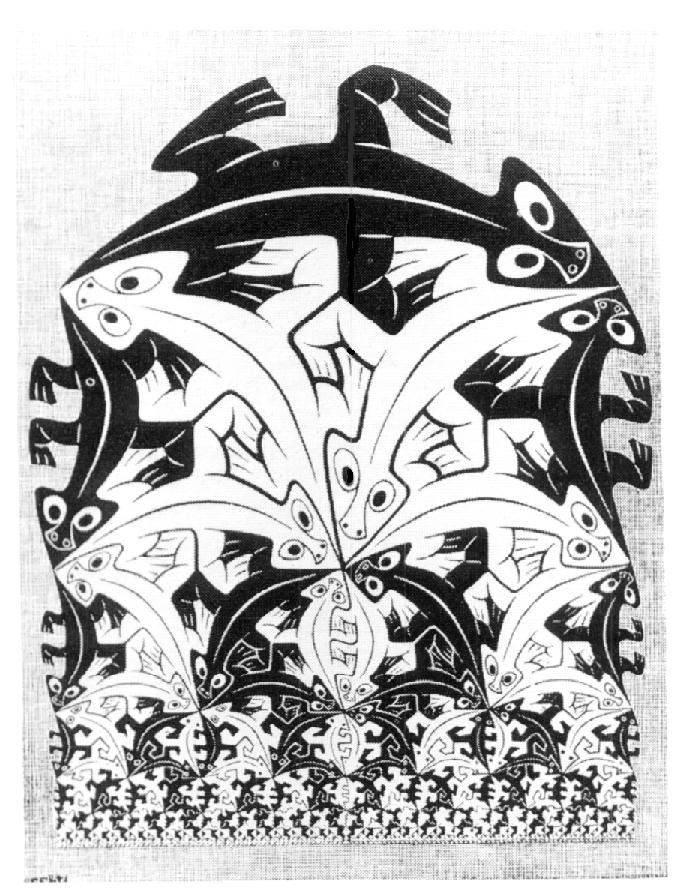
\includegraphics[width=150pt]{lizards.jpg}
\end{center}
\end{multicols}

\begin{rmk}
This is the equation for a {\em geodesic}, or shortest path, in an unusual geometry called the {\em hyperbolic upper-half plane}. The factor of $1/y$ in the integrand means that planar distances count for more towards the boundary of the upper-half plane (i.e. the $x$-axis) because $1/y$ gets very big when $y$ gets very small. This accounts for the warped shape of the ``straight lines'' in this geometry (which are now segments of circles centred on the $x$-axis) and gives rise to extremely pretty pictures like this one due to M. C. Escher.
\end{rmk}

\end{question}

\iffalse
\begin{answer}
Since $L$ has no explicit $x$-dependence, the Euler-Lagrange equation can be integrated up to give the Beltrami identity and we want to solve
\[L-y'\frac{\partial L}{\partial y'}=A,\]
\mks{1}
\begin{align*}
\Rightarrow\quad A&=\frac{\sqrt{1+(y')^2}}{y}-y'\frac{y'}{y\sqrt{1+(y')^2}}\\
&=\frac{1}{y\sqrt{1+(y')^2}}
\end{align*}
\mks{2}
which gives
\[y'=\sqrt{\frac{1}{y^2A^2}-1}\]
\mks{2}
Integrating, this gives
\begin{align*}x-C&=\int\frac{yAdy}{\sqrt{1-y^2A^2}}\\
&=-\sqrt{1-y^2A^2}/A\\
\Rightarrow&(x-C)^2+y^2=1/A^2\end{align*}
\mks{2}
which is the equation for a circle centred at $(C,0)$. Our geodesic is the segment of this circle between $x=a$ and $x=b$.
\end{answer}

\fi
\newpage

\begin{question}\ \\
Show that
\[y(x)=\cos^{-1}(A\cot x)+B\]
is the general solution to the Euler-Lagrange equation for the variational problem associated to the functional
\[\int\sqrt{1+(y')^2\sin^2x}dx.\]
{\em Hint: Use the two substitutions suggested by the solution!}
\begin{rmk}
The paths $\gamma(x)=(x,y(x)\cos x,y(x)\sin x)$ are shortest paths (``great circles'') on the unit sphere: the functional is just the length functional $\int|\dot{\gamma}(x)|dx$.
\end{rmk}
\end{question}

\bigskip

\iffalse
\begin{answer}
The Euler-Lagrange equation is
\[0=\dd{}{x}\pd{L}{y'}=\dd{}{x}\left(\frac{y'\sin^2x}{\sqrt{1+(y')^2\sin^2x}}\right)\]
so
\[\frac{y'\sin^2x}{\sqrt{1+(y')^2\sin^2x}}=C\]
for some constant $C$. This rearranges to give
\[(y')^2(\sin^2x-C^2)\sin^2x=C^2\]
or
\[y'=\frac{C}{\sin x\sqrt{\sin^2x-C^2}}.\]
Integrating gives
\[y=C\int\frac{dx}{\sin x\sqrt{\sin^2x-C^2}}\]
and this can be done by first substituting $u=\cot x$ ($du=-(1+u^2)dx$, $1+u^2=1/\sin^2x$) to get
\[y=-C\int\frac{du}{\sqrt{1-C^2-C^2u^2}}=-\int\frac{du}{\sqrt{(1-C^2)/C^2-u^2}}\]
and then substituting $u=\left(\sqrt{(1-C^2)/C^2}\right)\cos v$ ($du=-\left(\sqrt{(1-C^2)/C^2}\right)\sin vdv$) which gives
\[y=\int dv=v+B\]
and if $A=1/\sqrt{(1-C^2)/C^2}$ then $v=\cos^{-1}(Au)=\cos^{-1}(A\cot x)$, as required.
\end{answer}

\newpage
\fi

\begin{question}\ \\
Consider a function $x(t)$ describing the position at time $t$ of a particle of mass $m$ sitting in the force field $F$ whose strength is the gradient of a potential $-V(x)$. Find the Euler-Lagrange equation for the functional
\[\int_0^1\left(\dfrac{1}{2}m\dot{x}^2-V(x)\right)dt\]
and show that solutions obey Newton's law of motion $F=ma$. Interpret Beltrami's identity physically in this situation.
\end{question}

\bigskip

\iffalse
\begin{answer}
The Euler-Lagrange equation is
\[\pd{L}{x}=\dd{}{x}\pd{L}{\dot{x}}\ \Rightarrow\ -\dd{V}{x}=m\ddot{x}\]
which is precisely Newton's law given that $F=-\dd{V}{x}$ and $a=\ddot{x}$. Beltrami's identity becomes
\[C=L-\dot{x}\pd{L}{\dot{x}}=\dfrac{1}{2}m\dot{x}^2-V(x)-m\dot{x}^2=-(m\dot{x}^2+V).\]
The RHS is the total energy (kinetic plus potential) so Beltrami's identity tells us that energy is conserved (i.e. constant in time).
\end{answer}
\newpage
\fi

\begin{question}\ \\
Let $\gamma(t)=(t,t^2\cos(\theta(t)),t^2\sin(\theta(t)))$ be a parametric curve in $\RR^3$.
\begin{enumerate}
\item[(a)] Check that $\gamma(t)$ lies on the surface $S=\{y^2+z^2=x^4\}$.
\end{enumerate}
The length of this curve is defined to be the integral $\int|\dot{\gamma}(t)|dt$ where $\dot{\gamma}$ denotes the vector whose components are the $t$-derivatives of the components of $\gamma$.
\begin{enumerate}
\item[(b)] Write out this integral explicitly as a function of $t$ and $\dot{\theta}(t)$.
\item[(c)] Show that if $\theta$ solves the corresponding Euler-Lagrange equation (i.e. if $\gamma$ minimises length amongst paths on $S$) then
\[\theta(t)=\int\frac{C}{t^2}\sqrt{\frac{1+4t^2}{t^4-C^2}}dt\]
for some constant $C$.
\end{enumerate}
\end{question}

\iffalse
\begin{answer}
\begin{enumerate}
\item[(a)] We have $y^2+z^2=t^4(\cos^2\theta(t)+\sin^2\theta(t))=t^4=x^4$.
\item[(b)] The vector $\dot{\gamma}(t)$ is
\[(1,2t\cos\theta-t^2\dot{\theta}\sin\theta,2t\sin\theta+t^2\dot{\theta}\cos\theta)\]
which has length
\[\sqrt{1+4t^2+t^4\dot{\theta}^2}\]
so the curve has length
\[\int_0^1|\dot{\gamma}|dt=\int_0^1\sqrt{1+4t^2+t^4\dot{\theta}^2}dt.\]
\item[(c)] We compute the Euler-Lagrange equation for this integral, considered as a functional in $\theta$:
\[0=\frac{d}{dt}\frac{t^4\dot{\theta}}{\sqrt{1+4t^2+t^4\dot{\theta}^2}}\]
so
\[t^4\dot{\theta}=C\sqrt{1+4t^2+t^4\dot{\theta}^2}\]
for some constant $C$. This rearranges to give
\[\dot{\theta}=\frac{C}{t^2}\sqrt{\frac{1+4t^2}{t^4-C^2}}\]
as required.
\end{enumerate}
\end{answer}
\fi

\end{document}